% !TEX root = paper.tex

\section {Results}
\label{sec:results}
\subsection{$p_{\mathrm{T}}$ and multiplicity dependence}

\begin{figure}[h!]
		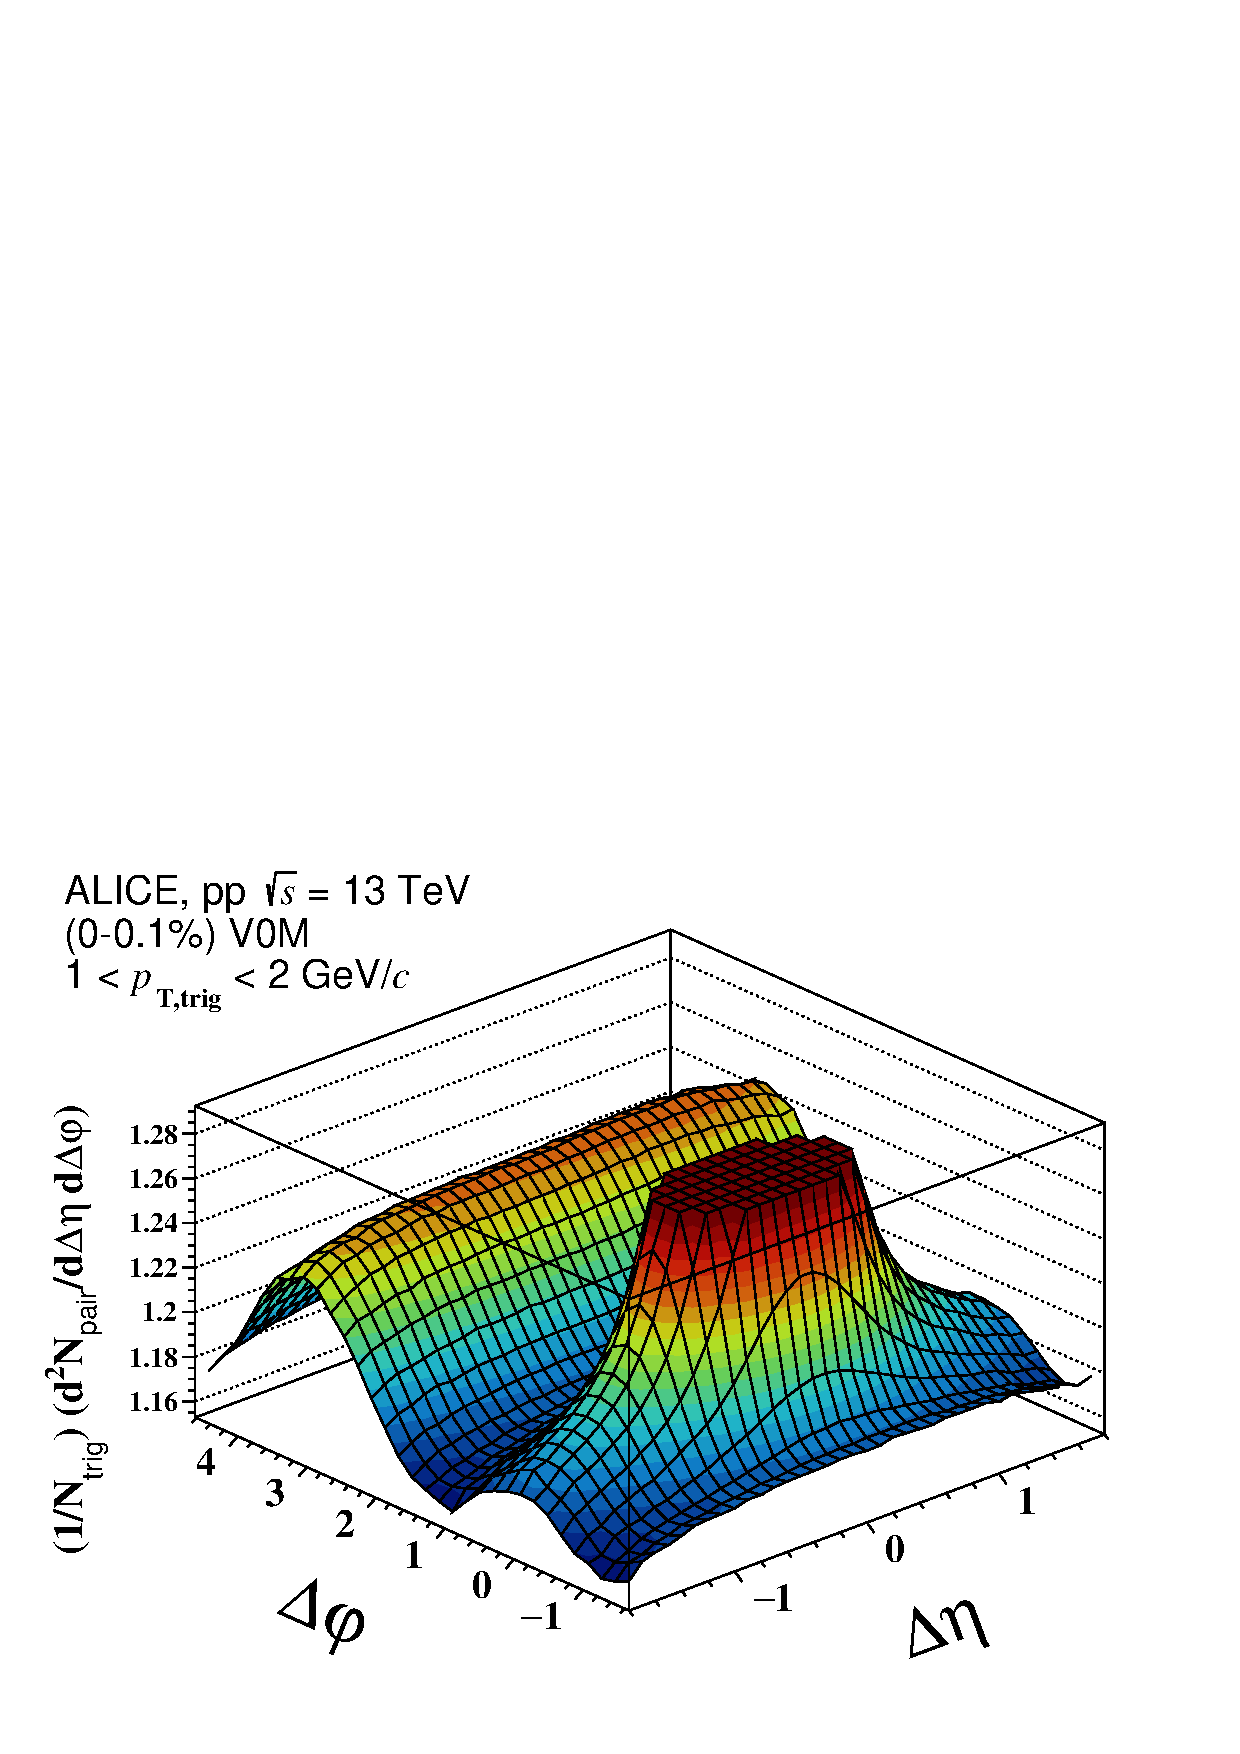
\includegraphics[width=0.33 \textwidth]{figures/CorrForAN_C_0_0_0_11.pdf} 
		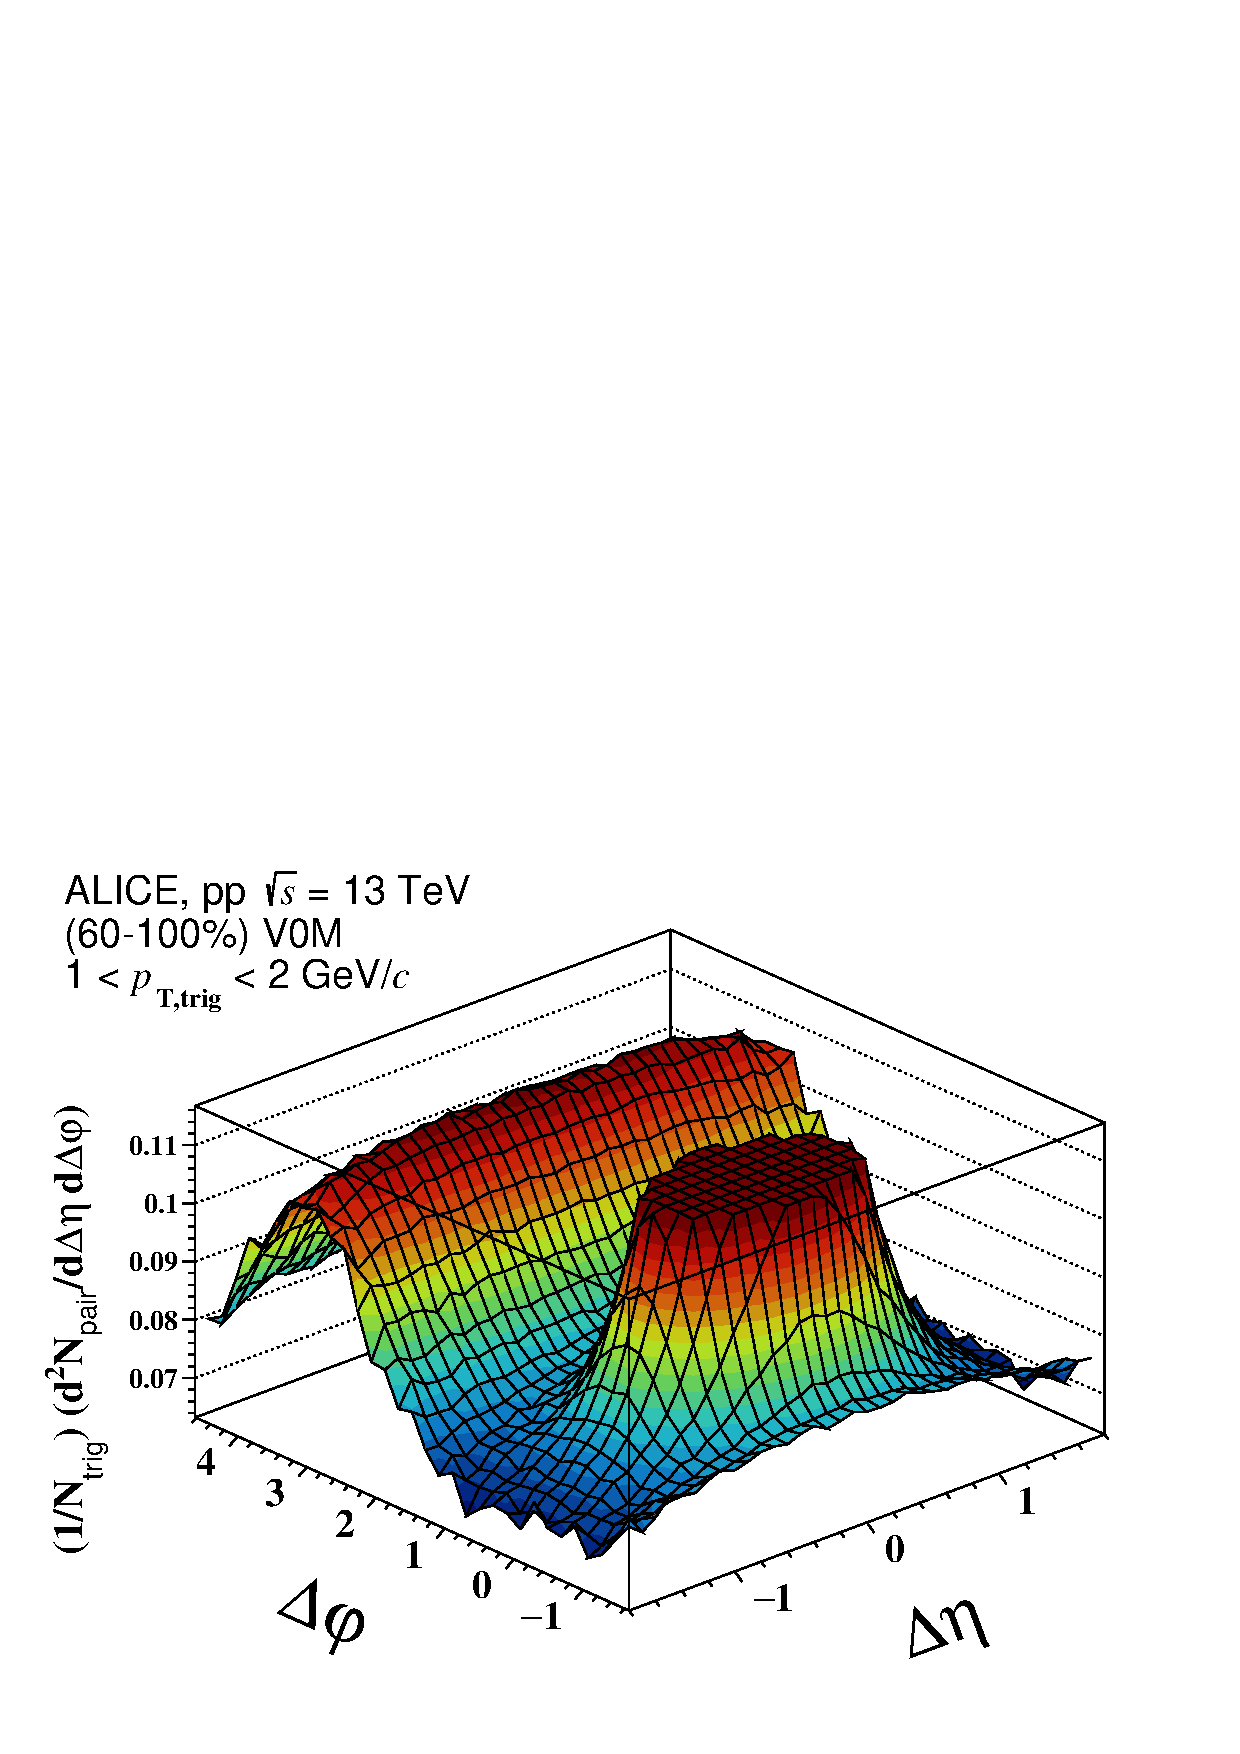
\includegraphics[width=0.33 \textwidth]{figures/CorrForAN_C_0_0_4_11.pdf} 
		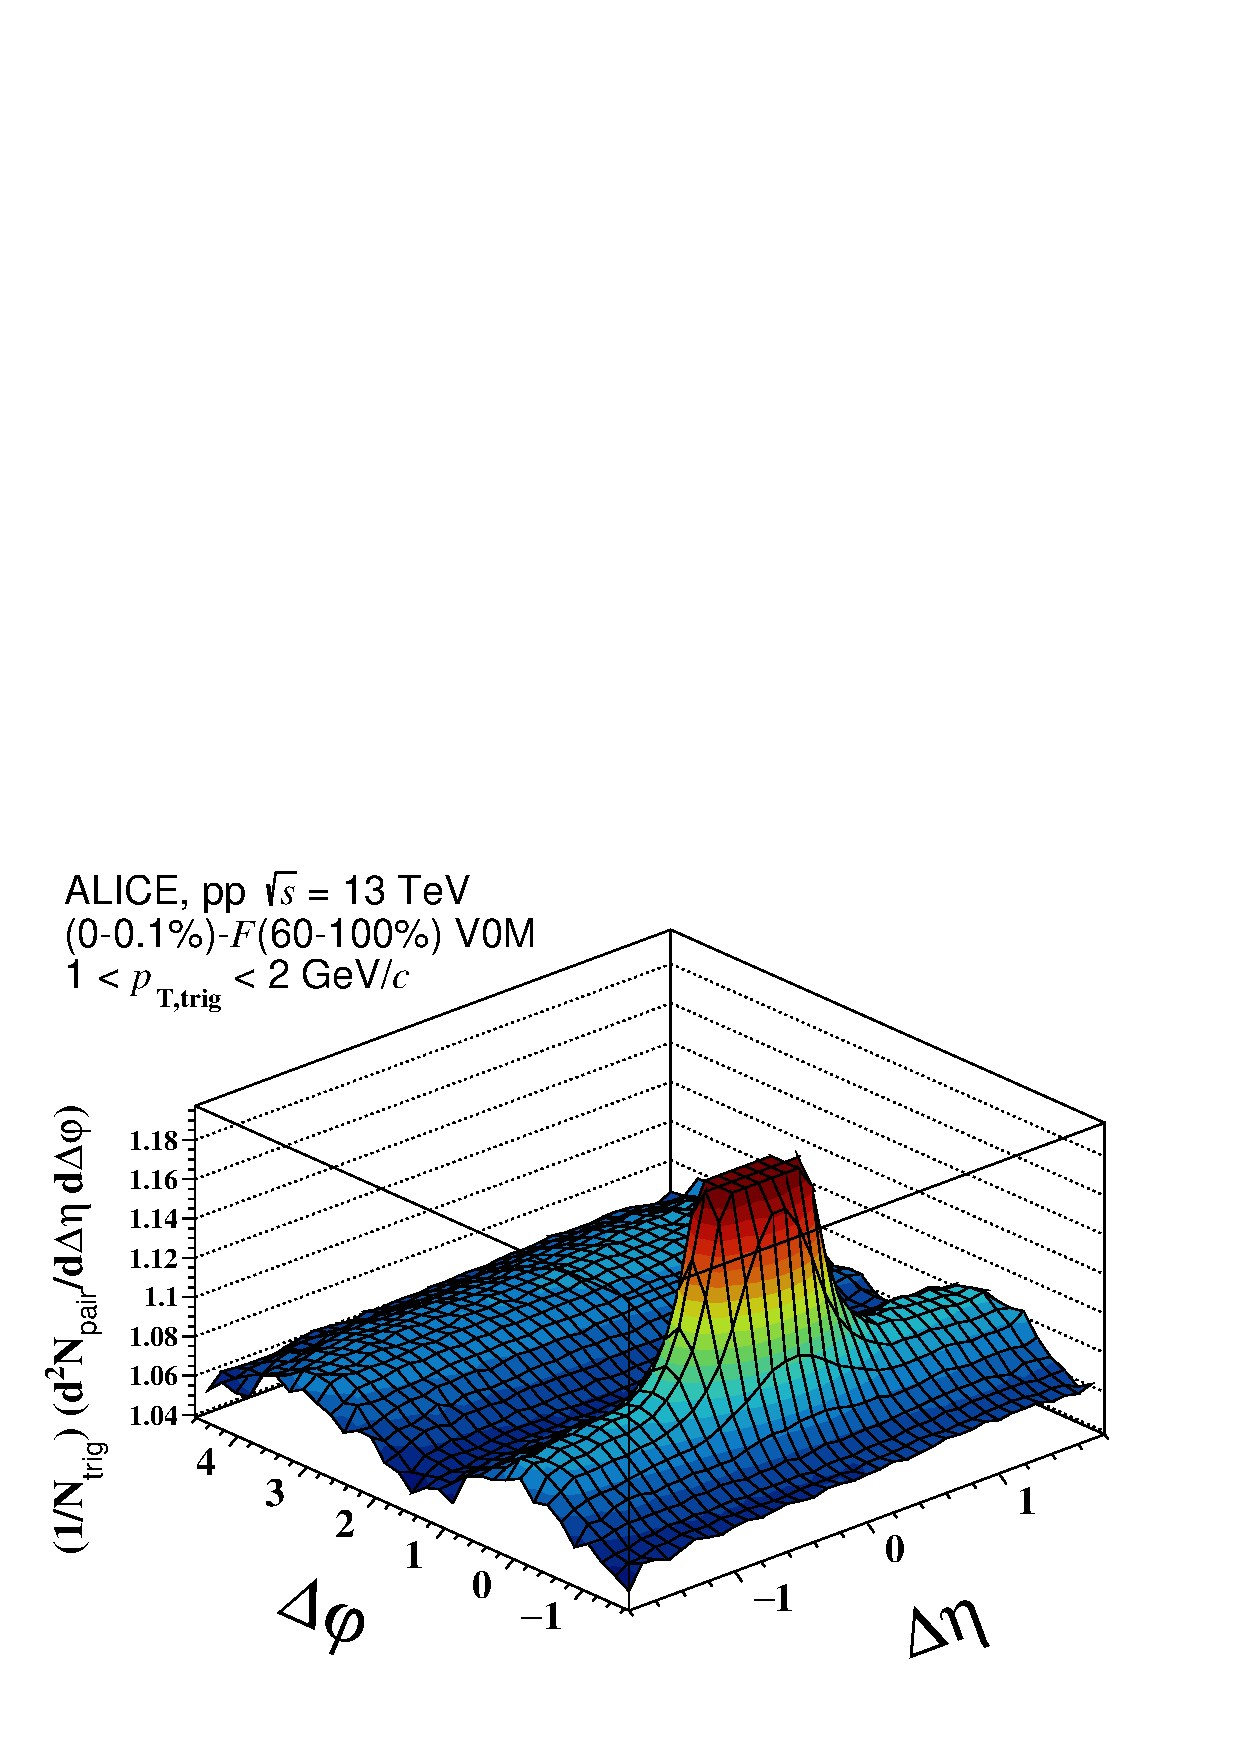
\includegraphics[width=0.33 \textwidth]{figures/CorrForAN_C_SUB_0_0_0_11.pdf} 
\caption{Two-particle correlation functions as functions of $\Delta\eta$ and $\Delta\varphi$ for HM(0--0.1\%, left) and LM(60--100\%, middle) events in $\sqrt{s}=13$ pp collisions. The subtracted one as (0--0.1)\%-$F$(60--100\%) is shown on the right. Note that the near-side jet peaks exceed the chosen range of the $z$-axis. The intervals of $\pttrig$ and $\ptassoc$ are 1~$<\it{p}_{\rm{T}}<$~2~GeV/$c$ in all cases.}
\label{fig:doubleridge}
\end{figure}
\begin{figure}[h!]
			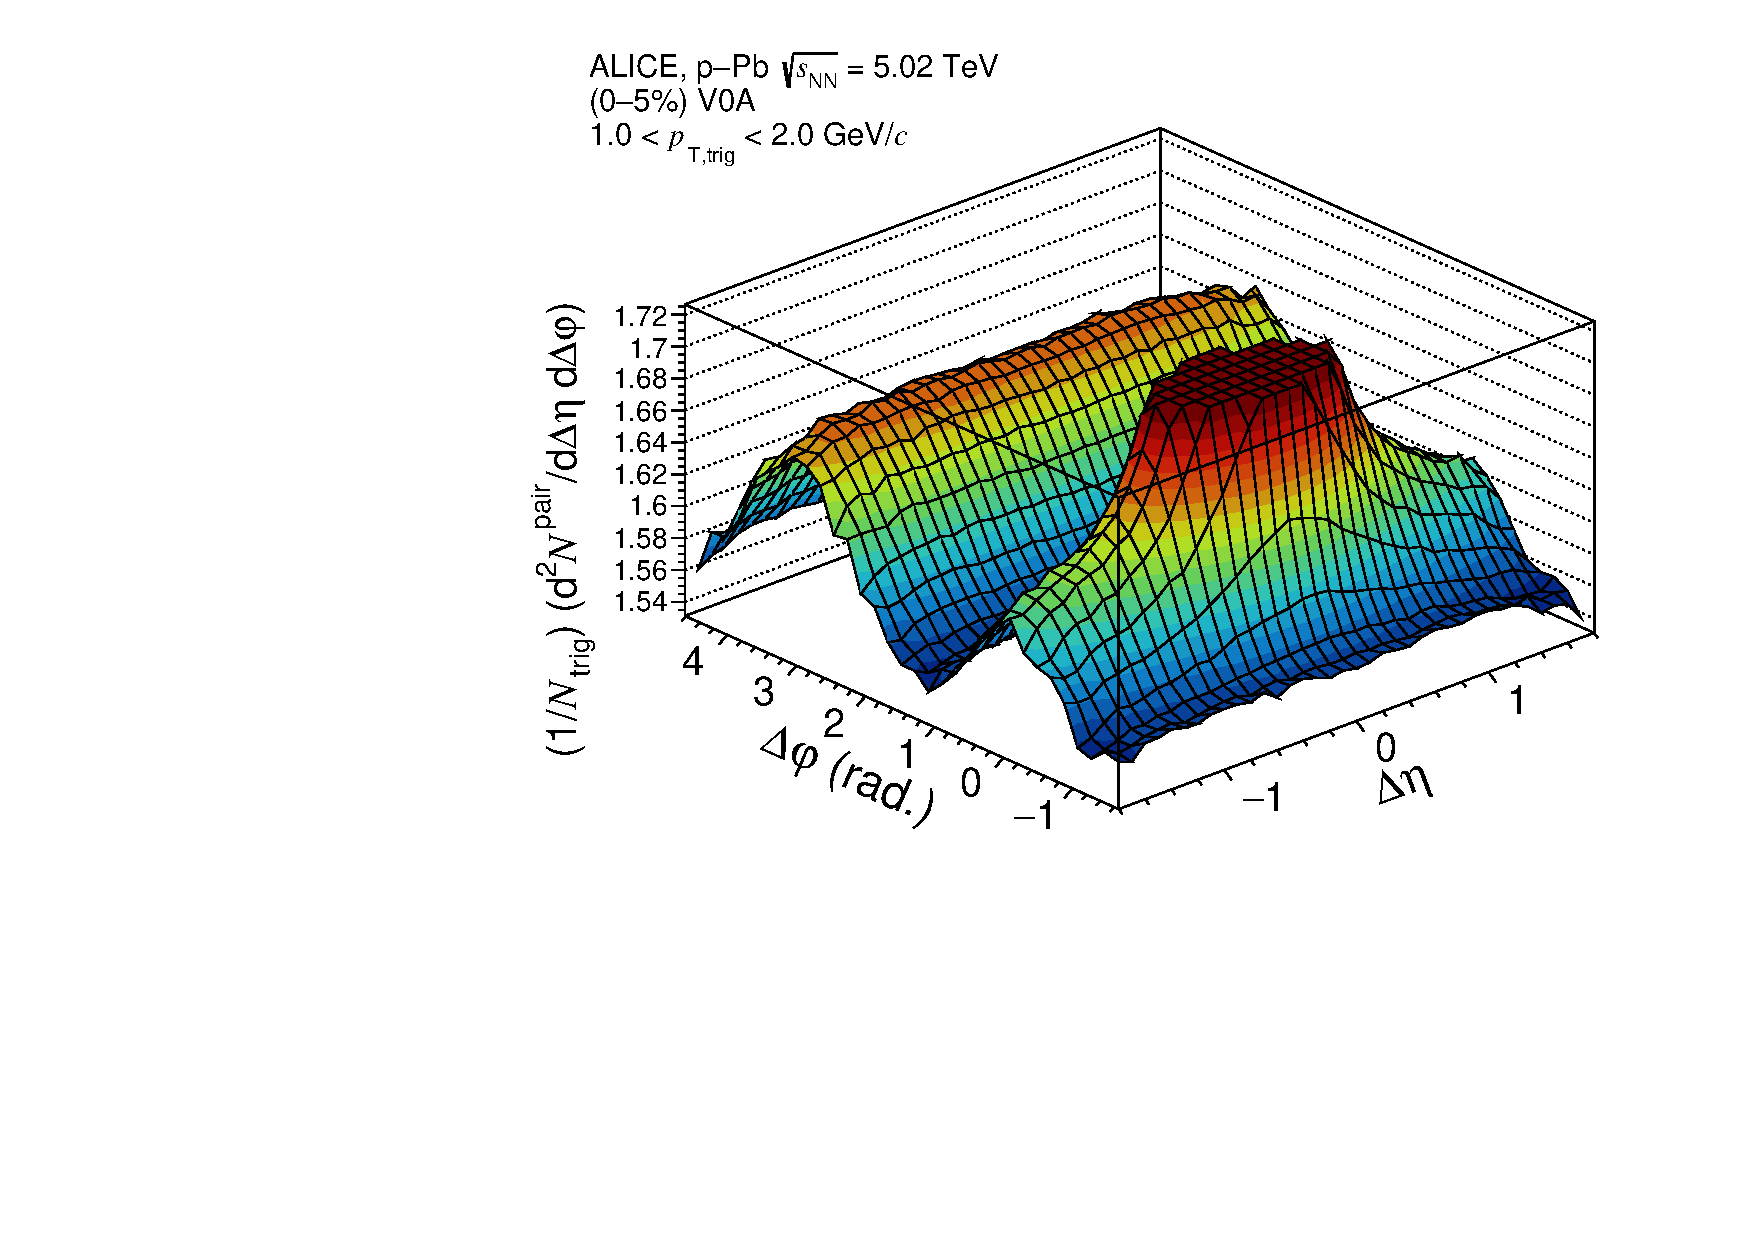
\includegraphics[width=0.33 \textwidth]{figures/corr_1_0_2_pPb.pdf}
			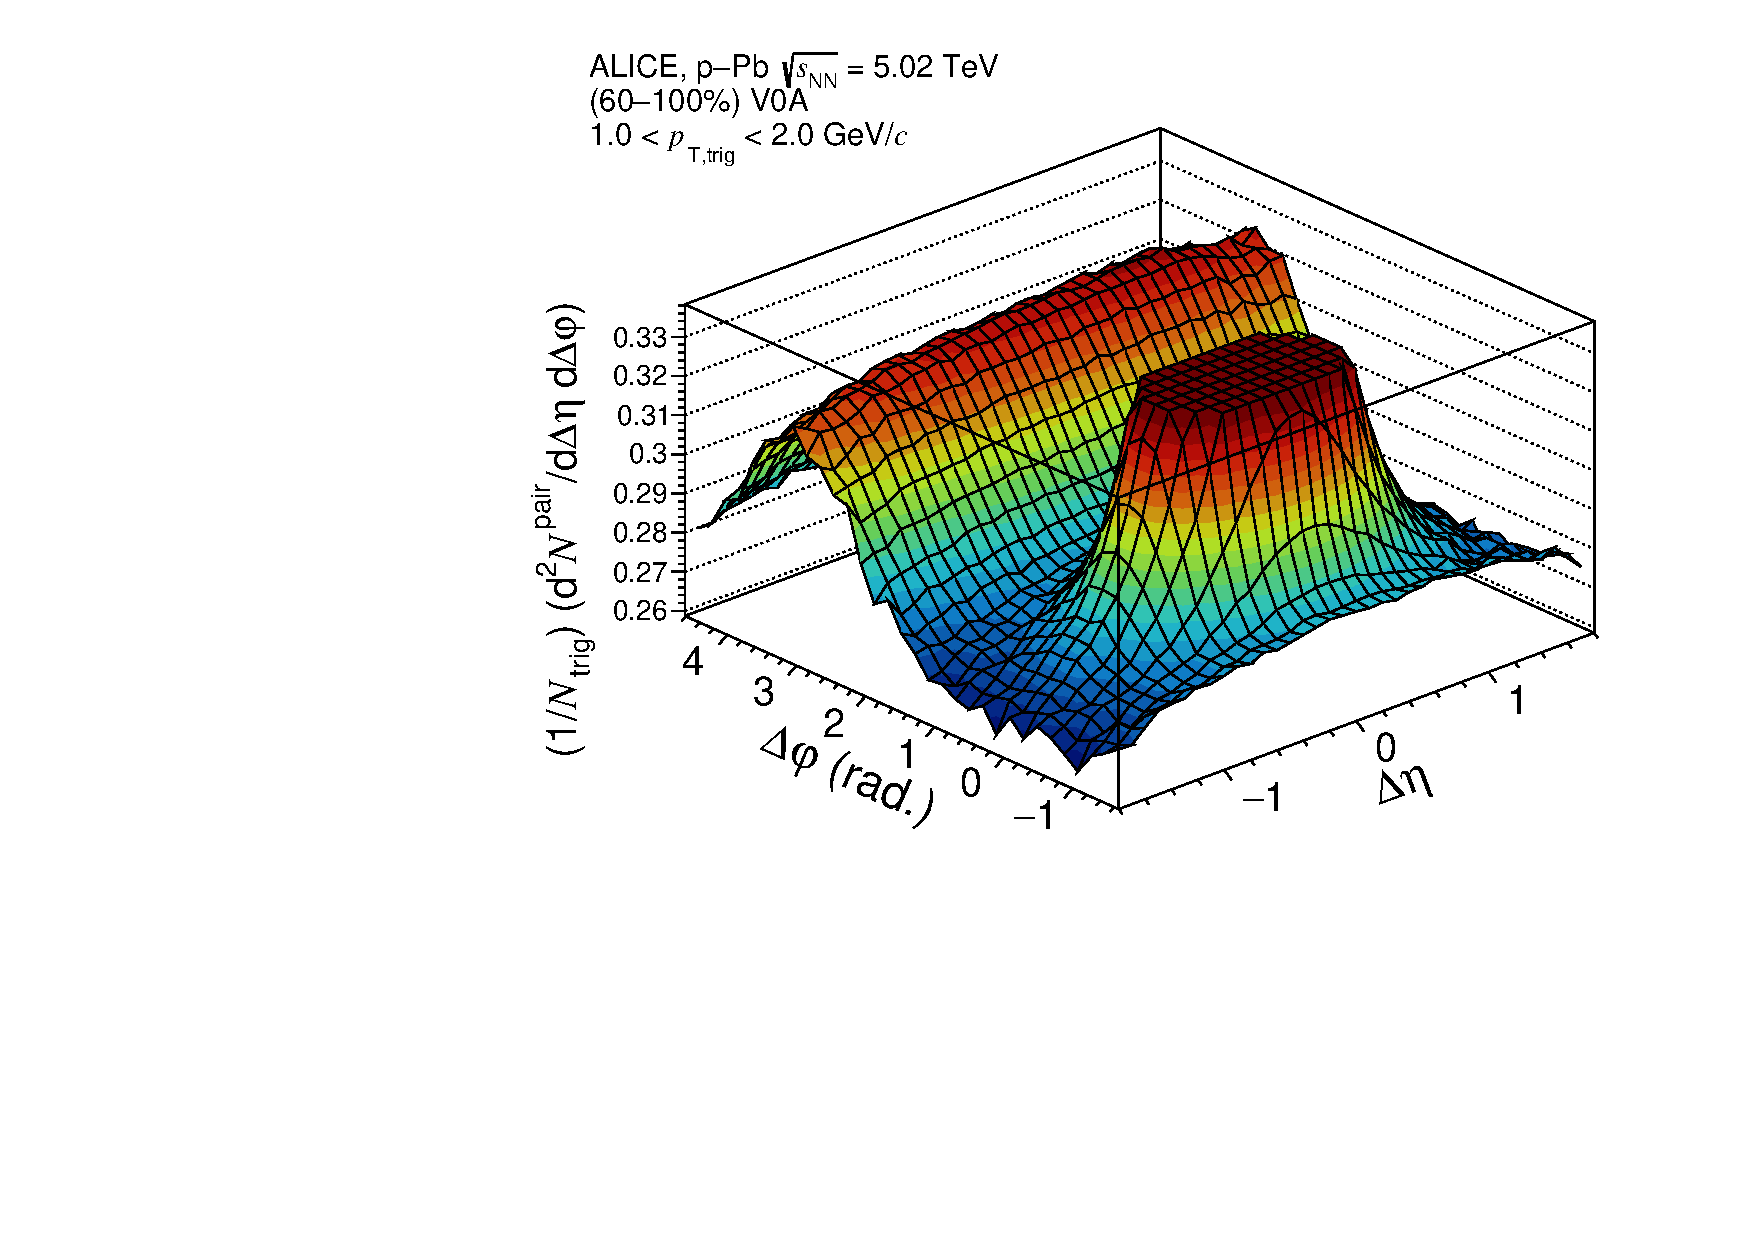
\includegraphics[width=0.33 \textwidth]{figures/corr_1_6_2_pPb.pdf}
			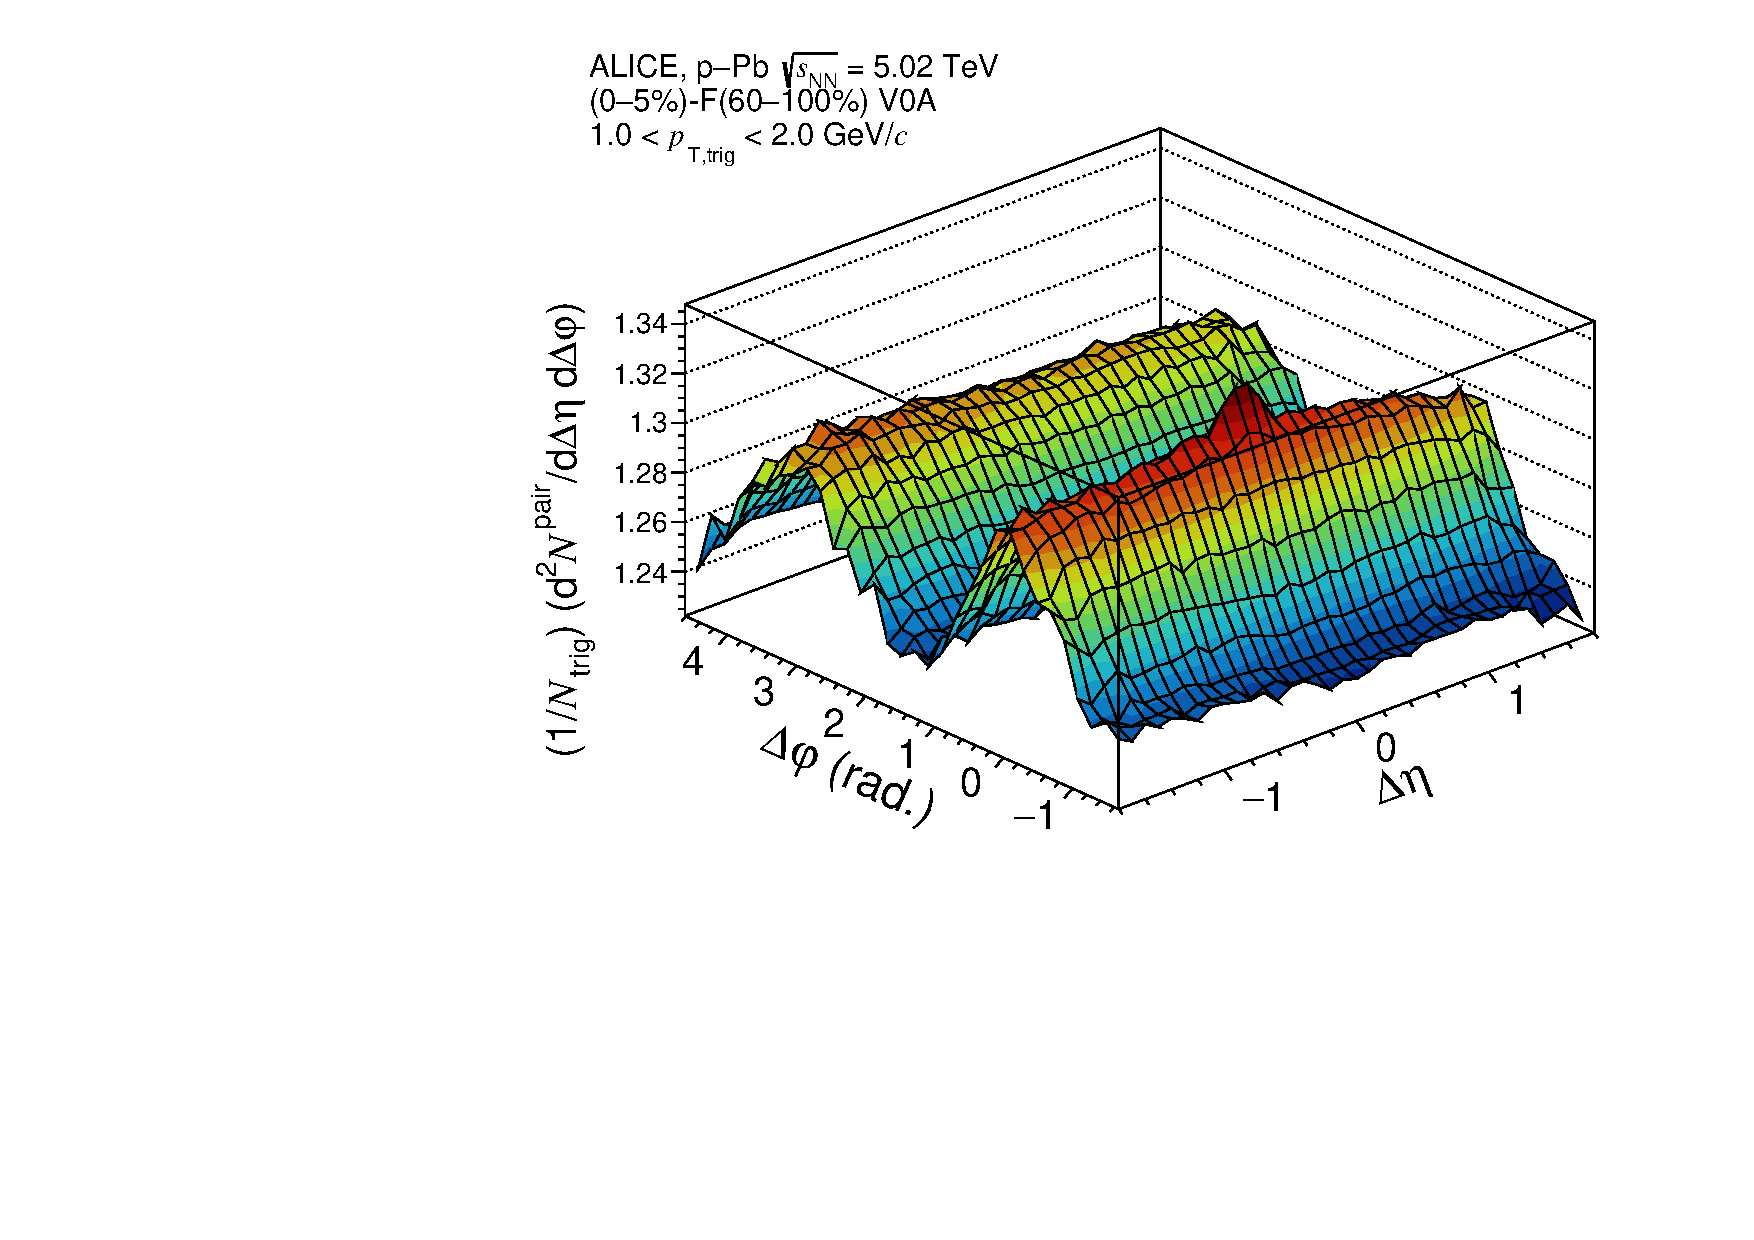
\includegraphics[width=0.33 \textwidth]{figures/corr_sub_fit_1_0_2_pPb.pdf}
\caption{Two-particle correlation functions as functions of $\Delta\eta$ and $\Delta\varphi$ for HM(0--5\%, left) and LM(60--100\%, middle) events in $\sqrt{s_{\mathrm{NN}}}=5.02$ TeV p-Pb collisions. The subtracted one as (0--5)\%-$F$(60--100\%) is shown on the right. Note that the near-side jet peaks exceed the chosen range of the $z$-axis. The intervals of $\pttrig$ and $\ptassoc$ are 1~$<\it{p}_{\rm{T}}<$~2~GeV/$c$ in all cases.}
\label{fig:doubleridgepPb}
\end{figure}

Two-dimensional correlation distributions in $\sqrt{s}=13$ TeV pp collisions are shown in Fig.~\ref{fig:doubleridge} for the high-multiplicity (0--0.1\%, left), low-multiplicity (60--90\%, middle), and the subtracted one as (0--5)\%-$F$(60--100\%) on the right. Similarly, the ones in $\sqrt{s_{\mathrm{NN}}}=5.02$ TeV p-Pb collisions are shown in Fig.~\ref{fig:doubleridgepPb}. The $F$ values can be found in Tab.~\ref{tab:Fpp} and \ref{tab:Fpb}, which come from the LM-template fit in a given multiplicity percentile as described in Sec.~\ref{sec:ana}. 
The $z$-axes for the yield of the correlations is properly scaled in order to zoom in the larger $\Delta\eta$ region, as a result, the jet peaks are sheared off in both figures. The flow modulations structure is clearly observed in the HM class while it is not seen in the LM-template. The away-side regions are populated mostly by back-to-back jet correlations for the HM and LM events but they are reduced and comparable to the one in near-side in $\Delta\eta > 1.6$. The jet peak in near-side region is remaining on the LM subtracted ones and the LM-template fit uses only $1.6< \Delta\eta < 1.8$.

\begin{figure}[h!]
	\centering
	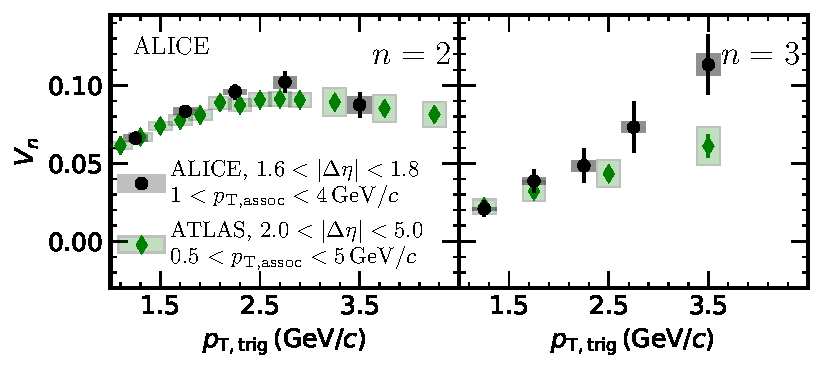
\includegraphics[width=0.8 \textwidth]{figures/Fig2_vn.pdf} 
	\caption{The magnitude of $v_2$ (left) and $v_3$ (right) as a function of $p_\mathrm{T}$. The results are compared to ATLAS measurements~\cite{Aaboud:2016yar}. Note that the event multiplicity definition, $p_{\mathrm{T},assoc}$ range, and $|\Delta\eta|$ acceptance are different.}
	\label{fig:vn}
\end{figure}

The extracted $v_2$ and $v_3$ are shown as a function of $p_{\mathrm{T},\mathrm{trig}}$ in Fig.~\ref{fig:vn}. These results are obtained from the $\sqrt{s}=13$ TeV pp LM-template fits for the high multiplicity percentile of $0-0.1\%$. The results are compared to ATLAS results~\cite{Aaboud:2016yar} where the same method was used to extract the flow coefficients. Even though the $\Delta\eta$ and $p_{\mathrm{T},\mathrm{assoc}}$ ranges are wider in the ATLAS results at $2.0<|\Delta\eta|<5.0$ and $0.5<p_{\mathrm{T},assoc}<5\,\mathrm{GeV}/c$, respectively, the results are consistent within the uncertainties. This is expected because the $\eta$ and multiplicity dependence of $v_n$ are expected to be small and $p_{\mathrm{T}}$ ranges are similar. Both results indicate that the overall magnitudes of the $v_n$ are larger at higher values of $p_{\mathrm{T},\mathrm{trig}}$, with maximum between $2.5<p_{\mathrm{T},\mathrm{trig}}<3.0$ GeV/c, which is similar to the results from Pb--Pb collisions~\cite{ALICE:2018yph}.

\begin{figure}[h!]
	\centering
	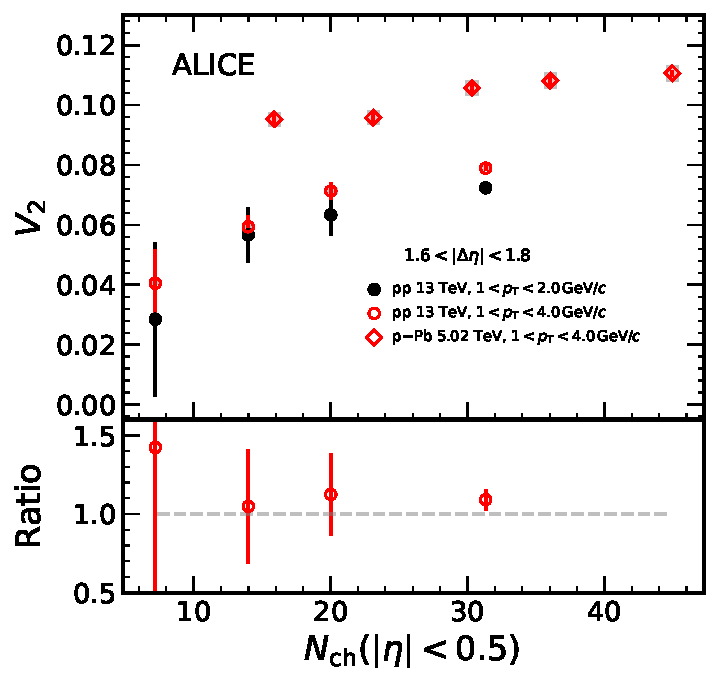
\includegraphics[width=0.55 \textwidth]{figures/Fig6_v2Mult_allSystemsComp2.pdf} 
	\caption{The $v_2$ magnitude for two different collision systems, pp and p-Pb, as a function of multiplicity in the mid-rapidity. Additionally, two different $p_\mathrm{T}$-intervals, $1.0<p_\mathrm{T}<2.0$ GeV/c and $1.0<p_\mathrm{T}<4.0$ GeV/c, are presented for pp collisions. The systems are differentiated with two different markers, circles and rhombuses, for pp and p-Pb respectively. The $p_\mathrm{T}$ intervals, are differentiated with different colored markers; black for $1.0<p_\mathrm{T}<2.0$ GeV/c and red for the $1.0<p_\mathrm{T}<4.0$ GeV/c. In the bottom panel, the ratio $1.0<p_\mathrm{T}<4.0$ interval over the $1.0<p_\mathrm{T}<2.0$ GeV/c interval is presented for pp-collisions and the statistical and systematic errors are combined in quadrature.} 
	\label{fig:v2mult}
\end{figure}

In Fig.\ref{fig:v2mult} the magnitude of $v_2$ as a function of multiplicity is presented for both pp and p--Pb collisions, at $\sqrt{s}=13$ and $\sqrt{s_\mathrm{NN}}=5.02$ TeV respectively. As in Fig.~\ref{fig:vn}, the large $\Delta\eta$ range is at $1.6<|\Delta\eta|<1.8$ and the $v_2$ is measured at $1<p_{\mathrm{T}}<4\,\mathrm{GeV}/c$ for both collision systems. Additionally, pp collisions at 13 TeV with $1<p_{\mathrm{T}}<2$ GeV/c is presented. Firstly, it is observed that the magnitude of $v_n$ increases with multiplicity for both collision systems and $p_\mathrm{T}$-ranges. Secondly, $v_2$ in p--Pb is higher than in pp collisions in the measured multiplicity range. These two are observed in Refs.~\cite{ATLAS:2015hzw,ATLAS:2016yzd, Khachatryan:2015lva}. 
%From~\cite{2016BSchenke} $v_n$ is expected to depend on the p--Pb collision geometry, however this dependence is not yet understood for pp collisions since by definition they  are only two colliding nucleons.
For the two different $p_\mathrm{T}$-interval presented for the pp collisions, $v_2$ in $1.0<p_\mathrm{T}<4.0$ GeV/c is larger than $v_2$ in $1.0<p_\mathrm{T}<2.0\,\mathrm{GeV}/c$. This agrees with what is observed in Fig.~\ref{fig:vn}, where the $v_2$ magnitude has its largest value between $2.5<p_\mathrm{T}<3.0\,\mathrm{GeV}/c$. The ratio of the higher to low $p_\mathrm{T}$ results is shown in the bottom panel of Fig.~\ref{fig:v2mult}, showing about $1\%$ increase within the uncertainties.


\subsection{Event-scale dependence}
\begin{figure}[h!]
	\centering
	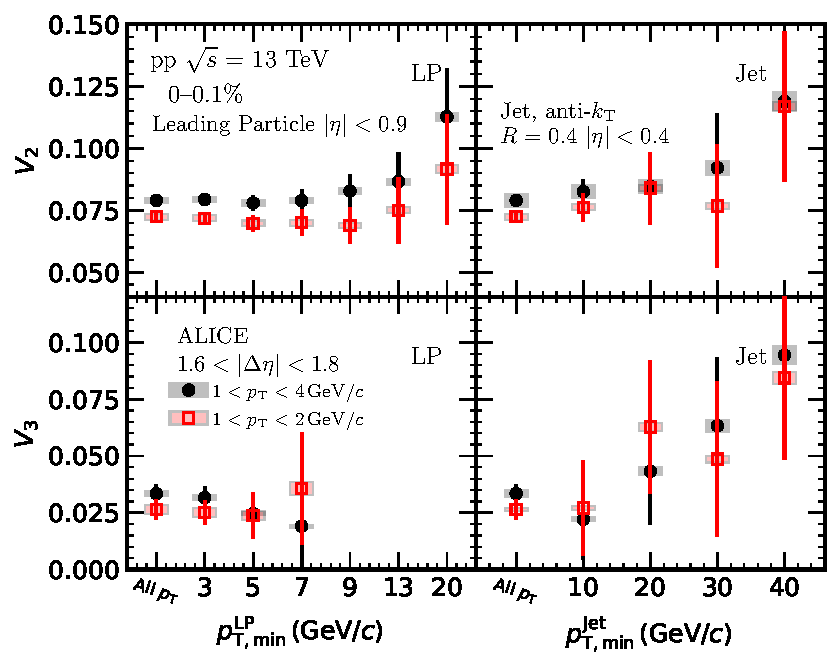
\includegraphics[width=0.6 \textwidth]{figures/Fig4_vn_LP.pdf}
	\caption{The magnitude of $v_2$ (top) and $v_3$ (bottom) as a function of the $\it{p}^{\rm{LP}}_{\rm{T,min}}$ (left) and $\it{p}^{\rm{jet}}_{\rm{T,min}}$ (right) in $\sqrt{s}=13$ pp collisions for $1<p_{\mathrm{T}}<2\,\mathrm{GeV}/c$ (red) and $1<p_{\mathrm{T}}<4\,\mathrm{GeV}/c$ (black). The filled circles and squares show measurement with ALICE. The statistical and systematic uncertainties are shown as vertical bars and boxes, respectively.}
	\label{fig:LPjet23}
\end{figure}    

Figure~\ref{fig:LPjet23} presents the extracted magnitude of $v_2$ and $v_3$ as function of the minimum $\ptlead$ ($\it{p}^{\rm{LP}}_{\rm{T,min}}$) and $\ptjet$ ($\it{p}^{\rm{jet}}_{\rm{T,min}}$) selections. Both event scale results are obtained from pp collisions at 13 TeV for the multiplicity class of $0-0.1\%$ and for two different $p_\mathrm{T}$-ranges, $1<p_{\mathrm{T}}<2\,\mathrm{GeV}/c$ in red and $1<p_{\mathrm{T}}<4\,\mathrm{GeV}/c$ in black . The leading particle is required to be within $|\eta|<0.9$ and the jets are reconstructed using the anti$-k_\mathrm{T}$ algorithm with R=0.4 and are required to be within $|\eta|<0.4$. $v_2$ and $v_3$ for both $p_\mathrm{T}$-ranges do not show any dependence on event-scale selection within the uncertainties, similarly for the ridge yields~\cite{ALICE:2021nir} and $v_{2}$ measurements  with a tagged $Z$ boson from the ATLAS collaboration~\cite{Aaboud:2019mcw}.
%The $\pythiashoving$ model describes the ridge yields qualitatively while the $\epos$ model overestimating the ridge yield.
While  EPOS LHC (PYTHIA8 String Shoving) model shows a strong (weak)  event-scale dependence and two models show different jet yields, it would be interesting to check how flow coefficients are related to the event-scale selections. However, up to date, it is not possible to extract flow coefficients with this LM-template method for these models because both models exhibit flow or ridge signals in LM events.

\section{Comparisons with models and other experiments}
\label{sec:theory}

\begin{figure}[h!]
	\centering
	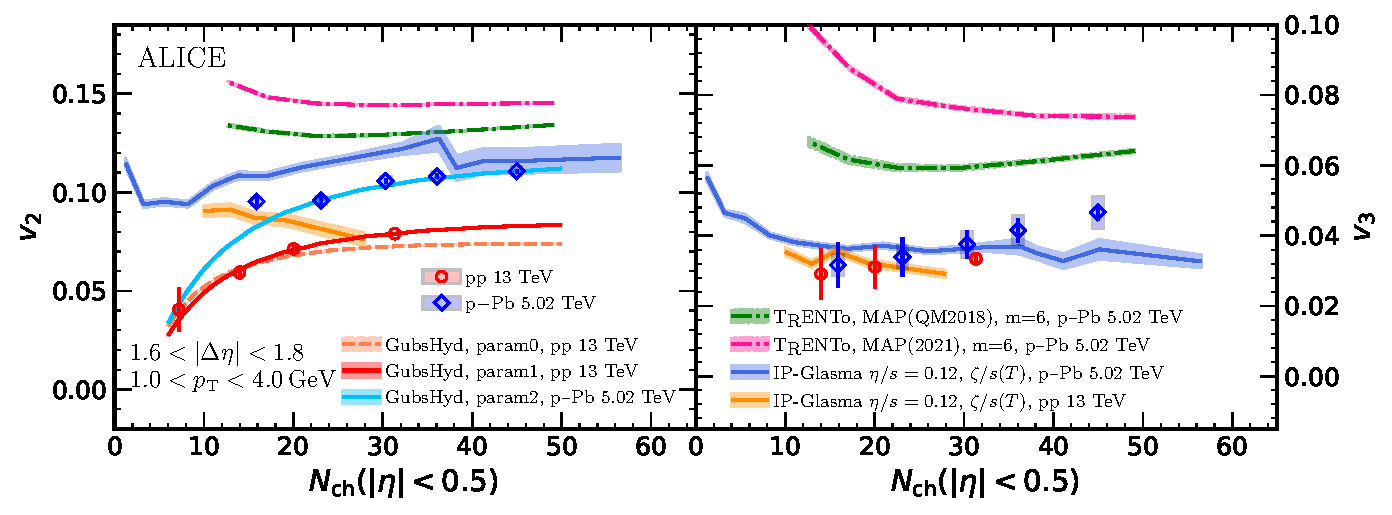
\includegraphics[width=0.9\textwidth]{figures/Fig6_v2Mult_allSystems_Hydro.pdf} 
	\caption{The $v_2$ (left) and $v_3$ (right) for p-Pb as a function of multiplicity in the mid-rapidity is compared to the hydrodynamic calculations. The blue and red markers represent the p--Pb and pp collision data points, respectively. The hydrodynamic calculations are presented with colored lines and bands marking their statistical uncertainty.} 
	\label{fig:vnmult_model}
\end{figure}

The results from p--Pb collisions are compared to the hydrodynamical calculations using the parametrization from an improved global Bayesian analysis using new sophisticated collective flow observables from two beam energies in Pb--Pb collisions~\cite{Parkkila:2021yha}. This hydrodynamic model, {T\raisebox{-.5ex}{R}ENTo}+iEBE-VISHNU, consists of the {T\raisebox{-.5ex}{R}ENTo} model~\cite{Moreland:2014oya} for the initial condition, which is connected with a free streaming to a 2+1 dimensional causal hydrodynamic model VISH2+1~\cite{Shen:2014vra}. The evolution is continued after particlization with a hadronic cascade (UrQMD) model~\cite{Bass:1998ca,Bleicher:1999xi}. The initial conditions, $\eta/s(T)$, $\zeta/s(T)$ and other free parameters of the hybrid model are extracted in a global Bayesian analysis.
%incorporating constraints measured from a Pb--Pb collision system at $\sqrt{s_\mathrm{NN}}=5.02\,\mathrm{TeV}$.
A model calculation with the best-fit parameterization for the transport coefficients chosen by maximum a posteriori (MAP) for Pb--Pb collisions at $\sqrt{s_{\text{NN}}}=5.02$~TeV as they are reported in Ref.~\cite{Parkkila:2021yha} is performed. The parameterization for the initial conditions, which include a the sub-nucleon structure with six constituent partons per nucleon, is taken from a model calibration with additional p--Pb data~[X]. All the kinematic cuts such as transverse momentum and pseudorapidity intervals are matched with the data reported in this article. The flow coefficients in the hydrodynamic calculation are extracted with the two-particle cumulant method, as the results are not affected by the away-side non-flow.

Figure~\ref{fig:vnmult_model} presents the model comparisons of the $v_2$ and $v_3$. It is found that {T\raisebox{-.5ex}{R}ENTo}+iEBE-VISHNU underestimates the data by large margin. Whereas the data shows a subtle centrality dependence with increasing values at larger multiplicities, {T\raisebox{-.5ex}{R}ENTo}+iEBE-VISHNU predicts low values at higher multiplicities and higher values and low multiplicities, similarly as is found in large collision systems~\cite{Acharya:2020taj}. The large discrepancies in the prediction can possibly be alleviated by inclusion of the newly measured p--Pb constraints in a future Bayesian parameter estimation, as well as by the improvement of the initial condition model for the small collision systems.

The results are also compared to IP-Glasma+MUSIC+UrQMD hydrodynamic calculations~\cite{Schenke:2020mbo}. This model uses IP-Glasma initial conditions~\cite{Schenke:2012wb} including sub-nucleonic fluctuations with three hot-spots per nucleon. The hydrodynamic evolution is performed by MUSIC~\cite{Schenke:2010rr} and coupled with the UrQMD~\cite{Bass:1998ca,Bleicher:1999xi} hadronic interactions. 
% mean-pT All paramters are fixed to reproduce 200 GeV Au+Au collisions at RHIC and 
The model calculations are performed with a constant $\eta/s=0.12$ and a temperature dependent $\zeta/s(T)$~\cite{Rose:2020lfc}. 
This model describes well the multiplicity dependence of $v_2$ in p--Pb collisions and the magnitude at the highest multiplicity but underestimates the data for lower multiplicity classes. As for pp collisions, the calculations clearly miss both the observed magnitude except for $N_{ch}>25$ as well as the trend of the multiplicity dependence. The model shows that $v_2$ decreases with increasing multiplicity, while the experimental result shows an increase.
%model missed important physics as the system becomes very small and the multiplicity very low, as is the case in p+p collisions, even though the initial T   does include initial state momentum anisotropies from the color glass condensate, as discussed in detail in [115]. arXiv:1908.06212 [nucl-th]. NEED to look further details.

%
\begin{figure}[h!]
	\centering
	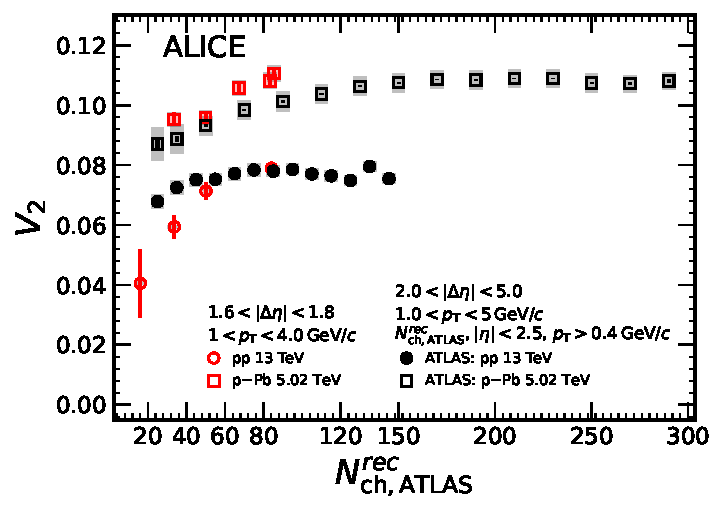
\includegraphics[width=0.45 \textwidth]{figures/Fig7_v2Mult_allSystemsATLAS.pdf} 
	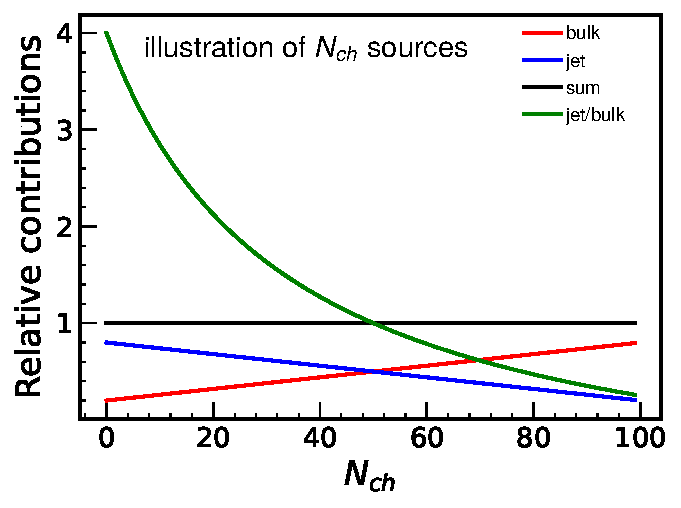
\includegraphics[width=0.425
	\textwidth]{figures/IllustrationNchSources.pdf} 
	\caption{Left: A comparison to ATLAS~\cite{Aaboud:2016yar} experiment of the $v_2$ magnitude for two different collision systems, pp and p-Pb, as a function of the ATLAS definition of multiplicity. Right:} 
	\label{fig:v2multATLAS}
\end{figure}

The multiplicity dependent $v_2$ measurements in Fig.~\ref{fig:v2mult} are compared with the results published by the ATLAS Collaboration~\cite{Aaboud:2016yar}. In case of the ATLAS measurement, the flow extraction method is slightly different from our analysis where a fit was performed after subtraction with a ZYAM assumption on the LM-template and the charged particle multiplicity was obtained by counting the number of reconstructed particles satisfying $\pt>0.4$~GeV/$c$ in $|\eta|<$~2.5. The ATLAS results have no efficiency correction (labeled as ${N^\mathrm{rec}_{\mathrm{ch},ATLAS}}$), therefore the result needs to take into account the efficiency reported in Ref~\cite{ATLAS:2016yzd}, which are 1.29 $\pm$ 0.05 and 1.18 $\pm$ 0.05 for the p--Pb and pp collisions, respectively. In our analysis, the reference multiplicity is measured by integrating the $\dndeta$ in $|\eta|<0.5$ for each multiplicity percentile measured by the V0M and V0A in pp and p--Pb collisions, respectively. 
The measured ALICE multiplicity percentiles are converted to the ATLAS definition by integrating the $\dndeta$ results for $\pt>0.4$~GeV/$c$ in their respective $\eta$-ranges using EPOS LHC simulation. 
The difference in multiplicity between the respective $\eta$-ranges, assuming that the $\eta$-distribution is flat. This is reduced to a factor of $\sim$three when requiring $p_\mathrm{T}>0.4$ GeV/c, i.e. a noticeable effect.
The EPOS LHC does not match with the measurements completely in $|\eta|<$~0.8 and it is scaled to the measurements before the integration. Based on the studies in \cite{ALICE:Nchpt}, the measured ALICE $\dndeta$ within $|\eta|<$~0.8 with various $\pt$ cut-offs are comparable to the measurements by ATLAS and CMS as well as EPOS LHC simulations. Finally, the comparison of our results to ATLAS is shown in Fig.~\ref{fig:v2multATLAS} as a function of ${N_\mathrm{ch}}^\mathrm{reco}$.  
Our results for p--Pb collisions agree with ATLAS in lower multiplicity and are slightly larger for our highest multiplicity interval. In case of  the pp collisions, our results agree better with the results by ATLAS for the highest two multiplicity intervals but are smaller at ${N^\mathrm{rec}_{\mathrm{ch},ATLAS}}<40$. The measured $v_{2}$ from both experiments decreases with decreasing multiplicity for both pp and p--Pb collisions, which is also predicted in hydrodynamic calculations~\cite{Weller:2017tsr,Taghavi:2019mqz}. Interestingly, the opposite is seen for pp collisions in Refs.~\cite{Schenke:2020mbo} as $v_2$ decreases with increasing
multiplicity. 
%Schenke:2020mbo
%the details of the initial state, including the initial flow profile and viscous stress tensor, missing
%the initial state momentum anisotropy is correlated with the observed elliptic flow in all small systems, with the effect increasing with decreasing multiplicity. 
As a lower bound for the size of a hydrodynamized
system where mainly the particles are emitted around the initial elliptic shape exists as predicted in Ref.~\cite{Taghavi:2019mqz}, there will be an transition of the flow signal but with the current experimental uncertainties and method it is still challenging to test its limit.


Another complication can arise from the different sources of the multiplicity between the models and data.  The previous mapping of ALICE multiplicity and ATLAS gives a naive way to compare the relative difference in multiplicities between two experiments but the measured $v_n$ might be averaged over different events. As illustrated in Fig.~\ref{fig:v2multATLAS} b, the relative jet (bulk) contribution depends on the measured $N_{ch}$. This results in lower $v_2$ value in average in low multiplicity events. While the data are compared to hydrodynamic model calculations, the difference in $N_{ch}$ should be taken into account carefully and this work need further thoughts.